\section{提案システム}
%第\ref{sec:related-works}で述べたように,これまでに提案されてきた検知に基づくDNS Tunneling対策には,Low Throughput手法および転送頻度を下げる手法に対して,検知が困難であるという課題がある.
%他方,新しいアーキテクチャに基づく名前解決システムには,マイグレーションの課題が残留している.
本章では,提案システムについて説明する.
はじめにシステムの概要と目的を示す.
次に,システムの詳細に関して,アーキテクチャ・動作メカニズム・プロトコル・スケーラビリティを順に説明する.

\subsection{フラットな名前空間に基づく名前解決システム : REFRES}
本節では,システムの概要について説明する.

REFRES(REcorded inFormation REsolution System)は,フラットな名前空間においてハッシュ値の範囲に基づきゾーンを分割し,そのゾーンを管理する主体として既存システムのTLDを割り当てることで,名前解決の手続きにおけるノードをクライアントとゾーン管理ノードのみに限定させた名前解決システムである.
REFRESでは,ドメイン名``www.example.com"のAレコードやドメイン名``www.example.com"のTXTレコードなど全てのレコード情報をフラットな名前空間上で管理する.
また,ドメイン名とリソースレコードタイプもしくはIPアドレスとリソースレコードタイプから算出されるハッシュ値を識別子とすることでレコード情報へのアクセスを実現する.
このようにして,REFRESにおけるクライアントは,レコード情報を保持するノードを一意に特定することができる.
具体的なレコード情報は,ゾーンを管理するサーバノードに階層的に連結したノードのよって作成・更新・破棄される.
レコード情報を操作する際には,事前に認証局との認証手続きをすることで,レコード情報の信頼を保証する.
最終的にREFRESでは,クライアントからの名前解決リクエストと偽装して送信される特定の権威サーバ指向の悪性クエリが発生する仕組みを抑止する.
REFRESの特徴を以下に示す.
\begin{itemize}
 \item フラットな名前空間
 \vspace{-3mm}
 \item ハッシュ値の範囲に基づくゾーニング
 \vspace{-3mm}
 \item レコード情報の操作と提供・管理の機能分離
 \vspace{-3mm}
 \item レコード情報に対する識別子の導入
 \vspace{-3mm}
 \item 全てのレコード情報が認証済み
\end{itemize}

\begin{figure}[t]
 \centering
 \label{fig:abstruct-REFRES-architecture}
 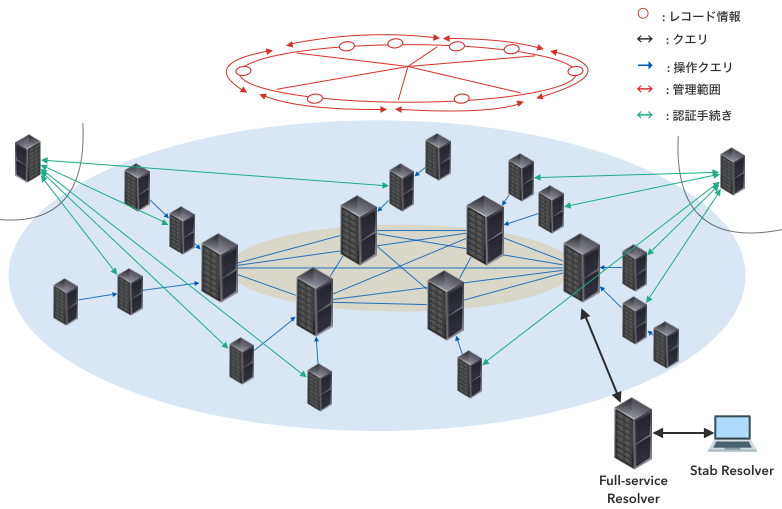
\includegraphics[scale=0.5]{figure/abstruct-architecture.png}
 \caption{REFRESの全体図}
\end{figure}


\subsection{デザイン}
\subsubsection{P2Pを組み合わせたハイブリッドなアーキテクチャ}
全体のアーキテクチャに関して,REFRESでは,既存のDNS同様にクライアントサーバアーキテクチャで構成される.
サーバは,フルメッシュネットワークで相互に接続される固定ノードによるP2Pネットワークアーキテクチャで構成される.


REFRESにおけるサービスノードは,機能に基づいて4つに分けることができる.
スタブリゾルバは,既存のDNSと同様に動作するノードであり,DNSクライアントとして名前解決を依頼する主体として位置づくノードである.
フルサービスリゾルバもスタブリゾルバ同様,1つ追加機能を除いて変更点はなく,スタブリゾルバからの問い合わせに対してリソース情報を保持する主体に代理的に問い合わせ機能と,問い合わせた情報を一定期間キャッシュするキャッシュサーバとして機能するノードである.
変更された点は,以降で説明するように,REFRESではレコード情報に対する識別子をキーとしてアクセスする.
フルサービスリゾルバは,スタブリゾルバからの従来のフォーマットのDNSクエリについて,ドメイン名とレコードタイプからハッシュ値の算出を行う機能を担う.
算出したハッシュ値をキーとして,フルサービスリゾルバは,サーバに転送する.
REFRESでは,権威サーバが機能に基づき二つサービスノードに分割される.

\begin{figure}[bh]
 \centering
 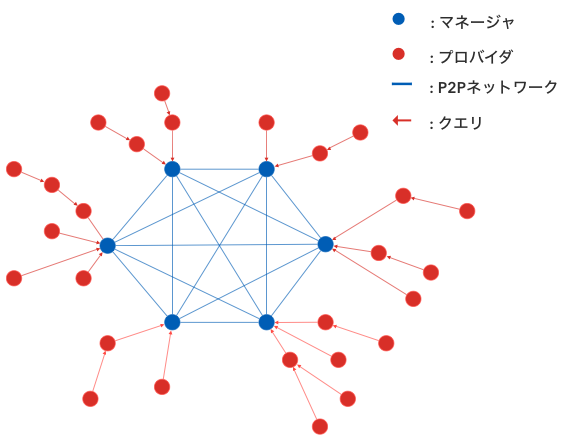
\includegraphics[scale=0.5]{figure/manager-provider.png}
 \caption{マネージャとプロバイダの関係図}
 \label{fig:manager-provider}
\end{figure}

マネージャは,実際のレコード情報を保持し,クライアントからの問い合わせに応答するサーバノードである.
また,マネージャは,既存のDNSにおけるTLDに位置づく権威サーバが担当する.
続いて,4つ目のサービスノードとなるプロバイダは,レコード情報を作成・更新および消去といった操作を担当する.
プロバイダは,既存のDNSにおけるSLD以降の権威サーバに相当し,ドメインの階層構造を従いマネージャに接続される.
プロバイダは,マネージャを介在することで,レコード情報を操作することができる.
例えば,example.comプロバイダが``www"のIPアドレス情報を作成することを考える.
example.comプロバイダは,``www.example.com"とレコードタイプ``A"およびその値``93.184.216.34"を含むデータを接続先のcomマネージャにリクエストする.
comマネージャは,リクエストされたドメイン名とそれに関連づけるレコードタイプから識別子を算出し,担当のマネージャにストアリクエストを転送するという具合で動作する.

%\begin{table}[htb]
 \centering
  \begin{tabular}{cc}
    \toprule
    表記 & 意味 \\
    \midrule
    フルサービスリゾルバ & リッスン \\
     &  管理
    \bottomrule
  \end{tabular}
 \label{tab:service}
 \caption{用語定義}
\end{table}


\subsubsection{ハッシュ関数に基づくレコード情報の識別子}
本節では,レコード情報に付与する識別子について説明する.
正引きの場合,従来のシステムでは,``ドメイン名"と``レコードタイプ"の二つの情報をキーとして,サーバは保持するゾーンファイルから該当するレコード情報の値が求まる.
REFRESでは,``ドメイン名"と``レコードタイプ"を表す文字列の和を引数として算出されるハッシュ値を識別子として利用することで,その識別子をキーに持つデータが求まる.
ドメイン名とそれに関連づけられたレコード情報の組み合わせについて,それら要素の文字列の和を引数としてハッシュ関数に適用することで,算出されるダイジェストを識別子として機能する構成となっている.

例えば,あるドメイン名に関連づけられたレコードタイプAのレコード情報について取得する場合を考える.
そのレコード情報が``com"サーバによって管理されているとき,クライアントは``com"サーバに対して識別子を含むリクエストパケットを転送することで,``com"サーバは識別子に対応するレコード情報をクライアントに応答するという具合である.

次に,識別子を算出する際に使用するハッシュ関数のアルゴリズムについて説明する.
(パケットフォーマット制約について説明)
DNSのパケットフォーマットは,5つのセクションに分類される.
(衝突強度について説明)
以上より,REFRESではパケットフォーマットに対する出力長と衝突に対する強度に基づき,224bitの名前空間をもつsha3アルゴリズムをハッシュ関数アルゴリズムとして用いる.

%また,あるドメイン名に対してレコード情報を関連づけたい場合,同様にしてドメイン名とリソースレコードのタイプの文字列和を引数として算出される識別子をキーとして,担当サーバに依頼することで,ハッシュテーブル上に情報がストアされる.

\subsubsection{ソートされたハッシュ空間の範囲に基づいたゾーン}
本節では,ゾーンの分割方法およびマネージャノードのアドレスとそのゾーンの範囲に関する対応表について説明する.
はじめに比較のために,従来のシステムの場合について説明する.
従来のシステムでは,ドメインの階層構造に従い,ドメインの管理ノードを下位のドメイン管理ノードに委譲することでゾーンが分割される.
この仕組みでは,ゾーン内の全てのレコード情報はゾーンファイルに画一的にまとめられ,そのゾーンを管理する権威サーバがレコード情報の保持機能とクライアントから応答するという二つの機能を担う.
このゾーン分割メソッドでは,レコード情報の帰属が明確であり,ドメインの管理ノードがトラストアンカーとしての役割を同時に担うことができるメリットがある.
一方のREFRESでは,識別子を算出する際に使用するハッシュ関数によって構成される名前空間に基づき,ソートされたハッシュの名前空間の連続した範囲で分割する.
この分割された連続した範囲に基づきゾーンがマネージャに割り当てられることで,既存システム同様にレコード情報全体を分散的に管理する.

上記で説明するように,マネージャが管理するゾーンは,ハッシュの名前空間の連続した一部の範囲である.
従って,レコード情報は,ハッシュの名前空間上で識別子をソートした際に,帰属する範囲を管理するマネージャによって保持される.
マネージャのアドレスを解決する方法には,ゾーンとしてハッシュ値の範囲とそのマネージャおよびマネージャのアドレスに関する対応表~\ref{tab:hash-management}によって解決される.
REFRESでは,フルサービスリゾルバ・マネージャ・プロバイダのノードがこの対応表を保持することで,識別子から一意にマネージャとそのマネージャのアドレスを特定する.
は,どのマネージャがどのハッシュ空間をゾーンとして管理しているのかに関する対応表を保持している.

\begin{table}[htb]
 \caption[マネージャとゾーンの対応表]{マネージャの情報とそのマネージャが管理するゾーンが記載された対応表の例}
 \centering
  \begin{tabular}{lrl}
    \toprule
		\multicolumn{1}{c}{\textbf{ゾーン}} & \begin{tabular}{c}\textbf{マネージャ}\\\textbf{アドレス}\end{tabular} & \multicolumn{1}{c}{\textbf{ドメイン}} \\
    \midrule
    (000…00, 2zz…zz) & 192.35.51.30 & com.  \\
		\multicolumn{1}{c}{...} & \multicolumn{1}{c}{...} & ... \\
    (500…00, 6zz…zz) & 192.5.6.30 & net. \\
		\multicolumn{1}{c}{...} & \multicolumn{1}{c}{...} & ... \\
    (b00…00, czz…zz) & 199.249.112.1 & org. \\
		\multicolumn{1}{c}{...} & \multicolumn{1}{c}{...} & ... \\
    (n00…00, mzz…zz) & 199.254.31.1 & info. \\
		\multicolumn{1}{c}{...} & \multicolumn{1}{c}{...} & ... \\
    (y00…00, zzz…zz) & 194.0.0.53 & arpa. \\
    \bottomrule
  \end{tabular}
 \label{tab:hash-management}
\end{table}


% ここで名前空間を分割するメカニズムを説明

\subsubsection{認証局によるレコード情報の認証基盤}
% 認証局を導入するとインターネットの匿名性を実現することが難しくなる
% レコード情報に認証局を導入する場合,webなどのサービスやコンテンツを提供するのが少し困難になる
% githubなどにおいては,同一ドメインにファイルという形でユーザにディスクを提供している
% CAを委譲する仕組みがある.これによって,
本節では,レコード情報の認証基盤について説明する.
REFRESでは,レコード情報の信頼性を担保するために,信頼できる第三者機関との認証プロセスをレコード情報のストアリングフェーズに介在させる.
REFRESにおけるレコード情報は,その情報の信頼性を担保するために,信頼できる第三者機関から発行される証明書を
REFRESでは,不審なレコード情報がハッシュテーブルにストアさせることを防ぐために,認証局モデルを採用する.
ために,全てのレコード情報をストアする前に認証局での評価を介在させる.
レコード情報をハッシュテーブル上にストアする前に認証局を介在させ,
ハッシュテーブル上にストアされるレコード情報に関して,認証機関を介在させることによって,プロバイダの真正性と不審なレコード情報をふるいにかける.

\subsubsection{強く型付けされたレコード情報}
本節では,REFRESで使用されるリソースレコードのタイプについて説明する.
第~\ref{sec:dns-infiltration}で示すように,既存のDNSで使用されるリソースレコードには,事前に特定のリソースレコードに対して任意の文字列を登録しておくことで外部からデータ転送のキャリアとして機能する特性がある.
本節では,DNS Infiltrationの対策を主たる目的として再構築したリソースレコードについて説明する.
% 強い型づけ


%\subsection{二重ハッシュ法と再帰問い合わせに基づくコリジョン対策}
% ここでコリジョンが発生した時のハンドリングについて説明する

\subsubsection{レコード情報のデータフォーマット}

\subsection{動作メカニズム}
\subsubsection{レコード情報に対する操作}
DNS Infiltrationに対応するため,リソースレコードを再定義する.
本節では,REFRESにおいて使用されるリソースレコードのタイプと
%TTLの更新方法について説明する

\subsubsection{名前解決}
%ハッシュテーブルのレプリケーション手法
%特定のハッシュ範囲を管理するノードは,複数用意させ,そのアドレスを対応表に明記し,ストアする際にその全てのレプリケーションサーバにストアリクエストする
%イベントドリブン
%非同期
